\documentclass[11pt,a4paper]{article}
\usepackage[T1]{fontenc}
\usepackage[utf8]{inputenc}
\usepackage[brazil]{babel}
\usepackage{lmodern}
\usepackage[margin=2.2cm]{geometry}
\usepackage{microtype}
\usepackage{graphicx}
\usepackage{float}
\usepackage{booktabs}
\usepackage{longtable}
\usepackage{array}
\usepackage{adjustbox}
\usepackage[font=small,labelfont=bf]{caption}
\usepackage{fancyvrb}
\usepackage{upquote}
\usepackage{xcolor}
\usepackage[colorlinks=true,linkcolor=blue!55!black,urlcolor=blue!55!black]{hyperref}
\usepackage{parskip}
\usepackage[colorlinks=true, linkcolor=blue, urlcolor=blue]{hyperref}

% Blocos de saída do notebook e de código para copiar.
\DefineVerbatimEnvironment{saida}{Verbatim}{fontsize=\scriptsize,frame=leftline,framerule=1.5pt,rulecolor=\color{gray!60},xleftmargin=4pt}
\DefineVerbatimEnvironment{codigo}{Verbatim}{fontsize=\footnotesize,frame=single,rulecolor=\color{gray!60}}

\emergencystretch=3em
\setlength{\LTpre}{6pt}
\setlength{\LTpost}{6pt}

\title{Etapa 1 --- Análise exploratória e diagnóstico da base}
\author{Equipe:\\[2pt]
Gabriel Egídio Santos Beloni\\
Gabriel Evangelista Massara\\
Pedro Henrique Cardoso Maia\\
Pedro Tinoco Lanna\\[4pt]
\small Disciplina de Inteligência Artificial --- Profa. Cristiane Neri Nobre\\
\small Trabalho em competição: Detecção de Intrusão em Redes (NSL-KDD)\\[4pt]
\small \textbf{Link Colab:} \href{https://colab.research.google.com/drive/1wmBIFtCfOWC75ihG_dJpAMJjheCWAftz?usp=sharing}{Acessar Notebook no Google Colab}\\
\small \textbf{Execução do Notebook:} \href{https://youtu.be/Qd1Tmvogv-A}{Assistir Vídeo no YouTube}}
\date{}
\begin{document}
\shorthandoff{"}
\maketitle

\tableofcontents
\clearpage
\section*{Como executar o notebook no Google Colab}
\addcontentsline{toc}{section}{Como executar o notebook no Google Colab}

Antes dos resultados, vale explicar como reproduzir a análise. O notebook usa um pacote escrito para este trabalho, o \texttt{nslkdd}, que fica na pasta \texttt{src/nslkdd/} do repositório. Por isso, abrir apenas o arquivo \texttt{.ipynb} no Colab não funciona: o ambiente precisa ter o projeto inteiro. O caminho mais simples é clonar o repositório no próprio Colab e dizer ao Python onde o pacote está.

\begin{center}\fbox{\parbox{0.92\linewidth}{\centering\textbf{Repositório a clonar:}\\\url{https://github.com/pedro-maia1337/IA-CopaLibertadores.git}}}\end{center}

\subsection*{Passo 1: abra o notebook}

Você pode abrir o \href{https://colab.research.google.com/github/pedro-maia1337/IA-CopaLibertadores/blob/main/notebooks/01_eda.ipynb}{notebook diretamente no Colab}. Se preferir, vá em \textbf{Arquivo > Abrir notebook > GitHub}, cole o endereço do repositório e escolha \texttt{notebooks/01\_eda.ipynb}.

\subsection*{Passo 2: envie a base de treino}

O clone não traz os dados, porque a pasta \texttt{data/new-database/} fica de fora do repositório. Abra o painel \textbf{Arquivos} do Colab, no ícone de pasta, e envie o \texttt{treino.csv} para \texttt{/content}.

\subsection*{Passo 3: prepare o ambiente}

Crie uma célula de código no topo do notebook, cole o trecho abaixo e execute. Ele clona o projeto, instala as bibliotecas, coloca a base no lugar certo e aponta o Python para a pasta \texttt{src/}:

\begin{codigo}
import os, sys
REPO = "/content/IA-CopaLibertadores"
if not os.path.isdir(REPO):
    !git clone https://github.com/pedro-maia1337/IA-CopaLibertadores.git {REPO}
%cd {REPO}
!pip install -q "scikit-learn>=1.6" "imbalanced-learn>=0.12"
!pip install -q "xgboost>=2.1" "shap>=0.46" "seaborn>=0.13"
!mkdir -p data/new-database
!cp /content/treino.csv data/new-database/
sys.path.insert(0, f"{REPO}/src")
\end{codigo}

\subsection*{Passo 4: confira se deu certo}

Em uma nova célula, logo abaixo, execute:

\begin{codigo}
from nslkdd import config
print(config.ROOT, config.TRAIN_FILE.exists())
\end{codigo}

Se tudo estiver certo, a resposta será:

\begin{saida}
/content/IA-CopaLibertadores True
\end{saida}

\subsection*{Passo 5: execute o notebook}

Agora é só usar \textbf{Ambiente de execução > Executar tudo}. Se o \texttt{pip} atualizar o numpy ou o pandas, reinicie a sessão e execute tudo de novo.

\subsection*{Alguns cuidados}

Não copie apenas a pasta \texttt{nslkdd/} para o Colab. O pacote descobre onde estão \texttt{data/} e \texttt{results/} a partir da posição de \texttt{src/nslkdd/config.py}, então ele precisa continuar dentro da estrutura do projeto. Pelo mesmo motivo, não use \texttt{pip install .}, que moveria o pacote para \texttt{site-packages}. Evite também o \texttt{requirements-lock.txt}, pois ele inclui o \texttt{pywinpty}, que só existe no Windows.

O Colab apaga \texttt{/content} quando a sessão termina, então baixe o que for gerado em \texttt{results/} antes de sair. Como as versões das bibliotecas podem ser diferentes das usadas aqui (Seção 0), alguns números podem variar um pouco. Por fim, \texttt{teste\_sem\_rotulo.csv} e \texttt{modelo\_de\_submissao.csv} só são necessários no notebook 04 e não devem ser enviados nos demais.

\section*{Resumo dos resultados}
\addcontentsline{toc}{section}{Resumo dos resultados}

A base tem 69.833 linhas e 50 colunas, e o problema é \textbf{binário}: separar conexões \texttt{normal} de \texttt{anomaly}. As anomalias são apenas 5,8\% das linhas, uma proporção de 16 para 1. Isso significa que um classificador que responde ``normal'' para tudo acerta 94\% das vezes e, ainda assim, tem F1-macro de só 0,485.

O achado mais importante é o \textbf{vazamento de dados}. As colunas \texttt{score\_ids\_legado}, \texttt{tipo\_alerta\_soc} e \texttt{tempo\_resposta\_analista\_min} são cópias ruidosas do rótulo: sozinhas, sem nenhum dado de rede, chegam a F1-macro 0,889, mais do que os 0,875 dos 41 atributos de rede (validação agrupada, F1-macro em todas as linhas, como a métrica oficial). Por isso, ficam \textbf{fora do modelo}. Outras 5 colunas novas são apenas cópias exatas de atributos existentes, com os mesmos ausentes, e também foram removidas.

A base também é ruidosa. Há 13.067 cópias de linhas (19\% do total) e 1.702 grupos em que a mesma linha aparece com os dois rótulos; cerca de 57\% desses conflitos parecem ser ataques reais. Além disso, 94\% das linhas têm algum valor ausente, em 24 atributos e com até 40\% de falta. Quase sempre essa falta parece aleatória, mas em \texttt{dst\_host\_serror\_rate} os valores altos somem mais, e são justamente eles que indicam ataque (ausência \textbf{MNAR}).

Por fim, 8\% das linhas têm valores impossíveis, sem relação com a classe, que tratamos como erro de medição. Os atributos \texttt{protocol\_type}, \texttt{flag} e \texttt{service} têm grafias variantes (96 $\rightarrow$ 67 serviços após padronizar). Como há tantas cópias, a validação cruzada precisa ser \textbf{agrupada}. A pontuação usa \textbf{todas as linhas}, como a métrica oficial; por causa dos conflitos, nem um classificador perfeito passaria de 0,905 de F1-macro.

\setcounter{section}{-1}

\section{Configuração e política de dados}

Usamos a semente \texttt{config.RANDOM\_STATE = 42} em todo o trabalho, para que os resultados possam ser repetidos. As versões das bibliotecas foram estas:

\begin{saida}
{'numpy': '2.5.4', 'pandas': '3.0.6', 'sklearn': '1.9.1', 'imblearn': '0.14.2', 'seaborn': '0.13.2'}
RANDOM_STATE = 42
\end{saida}

Nesta etapa, olhamos \textbf{apenas para \texttt{treino.csv}}. O arquivo \texttt{teste\_sem\_rotulo.csv} fica guardado para a submissão final, no notebook 04. A base original do NSL-KDD (\texttt{data/raw/}) também não é usada, porque contém as linhas do teste com os rótulos. Mesmo os limites de valores usados adiante vêm da definição dos atributos, e não do teste.

\section{Carga e visão geral}

Começamos lendo o arquivo bruto, para ver os dados como eles realmente chegam. Depois disso, passamos a usar \texttt{load\_train\_frame}, que padroniza o texto. O arquivo \texttt{treino.csv.pdf} é só a impressão do CSV e não acrescenta nada.

\begin{saida}
shape: (69833, 50)
memória: 41.4 MiB
\end{saida}

{\small
\begin{longtable}{lrrrrr}
\caption{Cinco primeiras linhas do arquivo bruto, com todas as 50 colunas. Linhas e colunas foram invertidas para caber na página.}\\
\toprule
coluna & linha 0 & linha 1 & linha 2 & linha 3 & linha 4 \\
\midrule
\endfirsthead
\multicolumn{6}{l}{\textit{(continuação da Tabela \thetable)}}\\
\toprule
coluna & linha 0 & linha 1 & linha 2 & linha 3 & linha 4 \\
\midrule
\endhead
\bottomrule
\endlastfoot
duration & 0 & 0 & 0 & 0 & 0 \\
protocol\_type & tcp & tcp & tcp & tcp & tcp \\
service & http & finger & http & smtp & http \\
flag & SF & SF & SF & SF & SF \\
src\_bytes & 219.0 & NaN & 162.0 & 942.0 & 232.0 \\
dst\_bytes & 3729 & 443 & 29122 & 332 & 479 \\
land & 0 & 0 & 0 & 0 & 0 \\
wrong\_fragment & 0 & 0 & 0 & 0 & 0 \\
urgent & 0 & 0 & 0 & 0 & 0 \\
hot & 0 & 0 & 0 & 0 & 0 \\
num\_failed\_logins & 0 & 0 & 0 & 0 & 0 \\
logged\_in & 1.0 & 0.0 & 1.0 & 1.0 & 1.0 \\
num\_compromised & 0.0 & 0.0 & 0.0 & 0.0 & NaN \\
root\_shell & 0.0 & 0.0 & 0.0 & 0.0 & 0.0 \\
su\_attempted & 0.0 & 0.0 & 0.0 & 0.0 & 0.0 \\
num\_root & 0 & 0 & 0 & 0 & 0 \\
num\_file\_creations & NaN & 0.0 & 0.0 & 0.0 & 0.0 \\
num\_shells & 0 & 0 & 0 & 0 & 0 \\
num\_access\_files & 0.0 & 0.0 & 0.0 & 0.0 & 0.0 \\
num\_outbound\_cmds & 0 & 0 & 0 & 0 & 0 \\
is\_host\_login & 0 & 0 & 0 & 0 & 0 \\
is\_guest\_login & 0 & 0 & 0 & 0 & 0 \\
count & 3.0 & 1.0 & 1.0 & 1.0 & 8.0 \\
srv\_count & 4.0 & 1.0 & 1.0 & 1.0 & 9.0 \\
serror\_rate & NaN & 0.0 & 0.0 & 0.0 & 0.0 \\
srv\_serror\_rate & 0.0 & 0.0 & 0.0 & 0.0 & 0.0 \\
rerror\_rate & 0.0 & 0.0 & 0.0 & 0.0 & 0.0 \\
srv\_rerror\_rate & 0.0 & 0.0 & 0.0 & 0.0 & 0.0 \\
same\_srv\_rate & 1.0 & 1.0 & 1.0 & 1.0 & 1.0 \\
diff\_srv\_rate & 0.0 & 0.0 & 0.0 & 0.0 & 0.0 \\
srv\_diff\_host\_rate & 0.50 & 0.00 & 0.00 & 0.00 & 0.22 \\
dst\_host\_count & 255.0 & 223.0 & 255.0 & 62.0 & 255.0 \\
dst\_host\_srv\_count & 255.0 & NaN & 255.0 & 173.0 & 255.0 \\
dst\_host\_same\_srv\_rate & 1.00 & 0.04 & 1.00 & 0.42 & 1.00 \\
dst\_host\_diff\_srv\_rate & NaN & 0.03 & 0.00 & 0.08 & 0.00 \\
dst\_host\_same\_src\_port\_rate & 0.00 & 0.00 & 0.00 & 0.02 & 0.00 \\
dst\_host\_srv\_diff\_host\_rate & 0.00 & 0.00 & 0.00 & 0.02 & 0.00 \\
dst\_host\_serror\_rate & 0.0 & 0.0 & NaN & 0.0 & NaN \\
dst\_host\_srv\_serror\_rate & 0.0 & 0.0 & 0.0 & 0.0 & 0.0 \\
dst\_host\_rerror\_rate & 0.0 & 0.0 & 0.0 & 0.0 & 0.0 \\
dst\_host\_srv\_rerror\_rate & 0.0 & 0.0 & 0.0 & 0.0 & 0.0 \\
src\_bytes\_kb & 0.213867 & NaN & 0.158203 & 0.919922 & 0.226562 \\
dst\_bytes\_kb & 3.641602 & 0.432617 & 28.439453 & 0.324219 & 0.467773 \\
total\_bytes & 3948.0 & NaN & 29284.0 & 1274.0 & 711.0 \\
same\_srv\_pct & 100.0 & 100.0 & 100.0 & 100.0 & 100.0 \\
protocolo\_cod & 0 & 0 & 0 & 0 & 0 \\
score\_ids\_legado & 0.176 & 0.067 & 0.245 & 0.239 & 0.231 \\
tipo\_alerta\_soc & OK & OK & OK & OK & OK \\
tempo\_resposta\_analista\_min & NaN & NaN & NaN & NaN & NaN \\
class & normal & anomaly & normal & normal & normal \\
\end{longtable}
}

Além dos 41 atributos do NSL-KDD, a base traz \textbf{8 colunas novas} que o enunciado não descreve. Não dá para confiar nelas sem investigar, e é isso que fazemos nas Seções 6 e 8.

\begin{saida}
papel
contagem/contínuo         17
taxa [0,1]                15
nova (não documentada)     8
binário                    6
categórico                 3
alvo                       1
\end{saida}

\begin{table}[H]
\centering
\caption{As 8 colunas novas.}
\begin{adjustbox}{max width=\linewidth}
\begin{tabular}{lrrrr}
\toprule
 & dtype & papel & n\_valores & ausentes\_\% \\
\midrule
src\_bytes\_kb & float64 & nova (não documentada) & 2114 & 40.0 \\
dst\_bytes\_kb & float64 & nova (não documentada) & 9147 & 0.0 \\
total\_bytes & float64 & nova (não documentada) & 8484 & 40.0 \\
same\_srv\_pct & float64 & nova (não documentada) & 88 & 5.1 \\
protocolo\_cod & int64 & nova (não documentada) & 3 & 0.0 \\
score\_ids\_legado & float64 & nova (não documentada) & 920 & 0.0 \\
tipo\_alerta\_soc & str & nova (não documentada) & 2 & 0.0 \\
tempo\_resposta\_analista\_min & float64 & nova (não documentada) & 1289 & 91.4 \\
\bottomrule
\end{tabular}
\end{adjustbox}
\end{table}

\section{Qualidade dos dados}

\subsection{Categorias com grafias diferentes}

Sem padronização, \texttt{TCP} e \texttt{tcp} seriam tratados como coisas diferentes:

\begin{table}[H]
\centering
\caption{Valores distintos antes e depois da padronização.}
\begin{adjustbox}{max width=\linewidth}
\begin{tabular}{lrr}
\toprule
 & bruto & padronizado \\
\midrule
protocol\_type & 6 & 3 \\
service & 96 & 67 \\
flag & 19 & 11 \\
\bottomrule
\end{tabular}
\end{adjustbox}
\end{table}

Essa correção é uma regra fixa: ela não aprende nada com os dados e não remove linhas. Por isso, pode ser aplicada já na carga, do mesmo jeito no treino e no teste.

\subsection{Valores ausentes}

\begin{figure}[H]
\centering
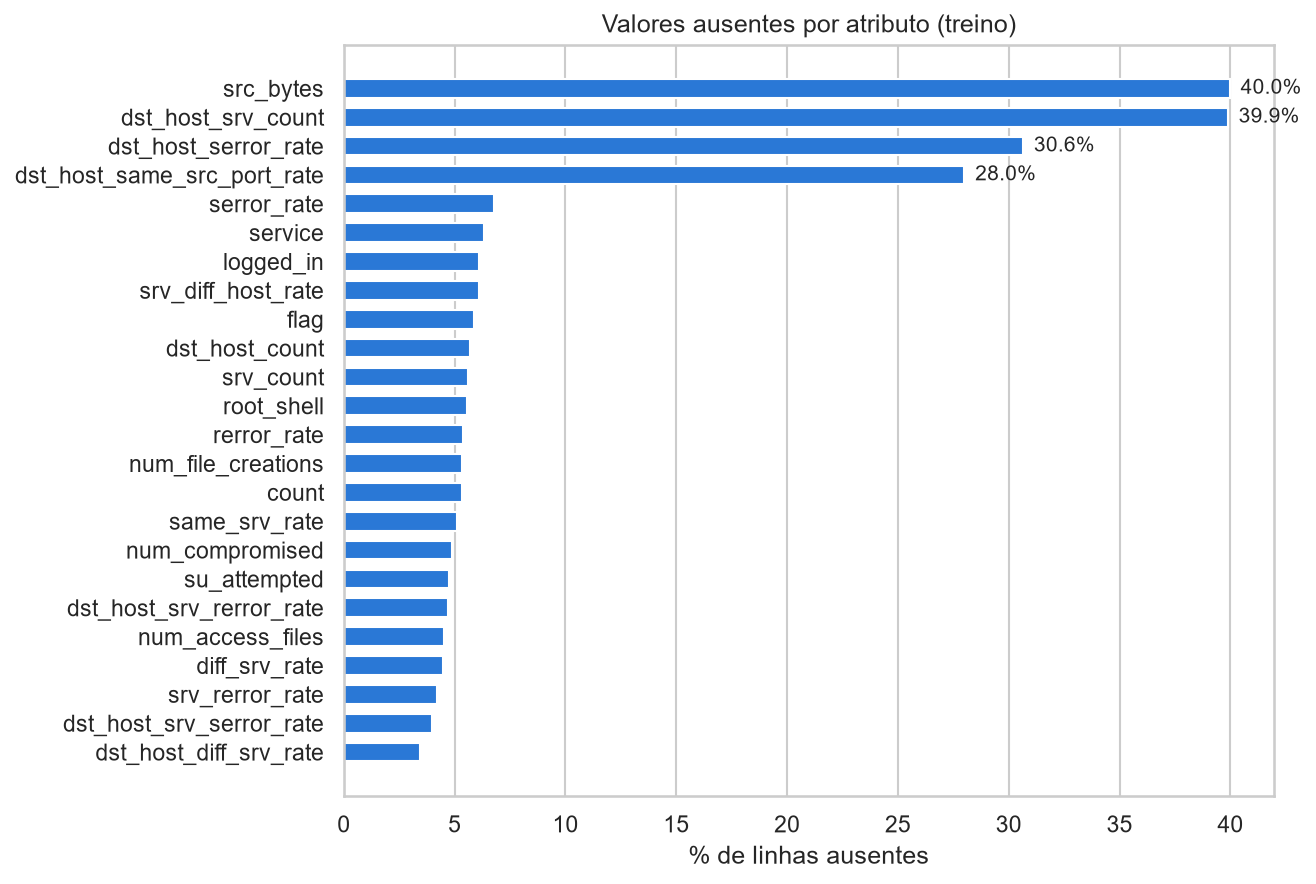
\includegraphics[width=6.50in,height=0.40\textheight,keepaspectratio]{figuras/eda_ausentes.png}
\caption{Percentual de ausentes por atributo.}
\end{figure}

\begin{saida}
24 de 41 atributos têm ausentes; 93.8% das linhas têm ao menos um.
\end{saida}

Quase toda linha tem algum valor faltando, então \textbf{descartar linhas não é uma opção}. Além disso, o teste também tem ausentes e não pode perder linhas, ou seja, o modelo precisa saber lidar com essa falta.

\subsection{Por que os valores faltam?}

Se a chance de um valor faltar depende da classe, a própria ausência é uma informação útil. Se não depende, é só ruído. Medimos isso comparando a taxa de anomalia com e sem o valor:

\begin{table}[H]
\centering
\caption{Taxa de anomalia com e sem ausente, por atributo.}
\begin{adjustbox}{max width=\linewidth}
\begin{tabular}{lrrrrr}
\toprule
 & atributo & ausentes\_\% & anomaly\_se\_ausente\_\% & anomaly\_se\_presente\_\% & razao \\
\midrule
21 & dst\_host\_serror\_rate & 30.6 & 8.5 & 4.6 & 1.85 \\
10 & num\_file\_creations & 5.4 & 6.5 & 5.8 & 1.12 \\
18 & service & 6.3 & 6.2 & 5.8 & 1.07 \\
1 & dst\_host\_srv\_serror\_rate & 4.0 & 6.1 & 5.8 & 1.05 \\
4 & num\_access\_files & 4.5 & 6.1 & 5.8 & 1.05 \\
\bottomrule
\end{tabular}
\end{adjustbox}
\end{table}

\begin{saida}
P(dst_host_serror_rate ausente) por faixa de dst_host_srv_serror_rate:
dst_host_srv_serror_rate
0              0.303
(0; 0,5]       0.251
(0,5; 0,99]    0.250
(0,99; 1]      0.527
\end{saida}

Na maioria dos atributos, a falta parece aleatória (MCAR). A exceção é \texttt{dst\_host\_serror\_rate}, um caso \textbf{MNAR}: quando ele falta, a taxa de anomalia quase dobra, e a ausência sobe de cerca de 30\% para 53\% quando o erro SYN é máximo. Em outras palavras, os valores altos tendem a sumir, e valores altos indicam ataque.

Isso tem uma consequência prática: preencher com a média ou a mediana apagaria esse sinal, colocando um valor baixo justamente onde ele deveria ser alto. Por isso, a Etapa 2 vai comparar o tratamento nativo de NaN com o indicador de ausência (\texttt{median\_indicator}).

\subsection{Valores impossíveis}

Alguns valores simplesmente não podem existir. Taxas ficam entre 0 e 1, \texttt{count} e \texttt{srv\_count} vão até 511, \texttt{dst\_host\_*} para em 255 e nenhum atributo numérico pode ser negativo. Mesmo assim, encontramos violações:

\begin{table}[H]
\centering
\caption{Valores acima do limite e negativos, por atributo.}
\begin{adjustbox}{max width=\linewidth}
\begin{tabular}{lrr}
\toprule
 & acima\_do\_limite & negativos \\
\midrule
dst\_host\_count & 912 & 0 \\
dst\_host\_srv\_diff\_host\_rate & 739 & 0 \\
dst\_host\_srv\_rerror\_rate & 714 & 0 \\
rerror\_rate & 683 & 0 \\
dst\_host\_same\_srv\_rate & 670 & 0 \\
dst\_host\_diff\_srv\_rate & 623 & 0 \\
srv\_count & 507 & 0 \\
count & 464 & 0 \\
duration & 24 & 358 \\
src\_bytes & 0 & 189 \\
\bottomrule
\end{tabular}
\end{adjustbox}
\end{table}

\begin{saida}
linhas com ao menos um valor impossível: 5674 (8.1%)
taxa de anomalia nessas linhas: 0.059 | nas demais: 0.058
valores das taxas acima de 1: [np.float64(1.5), np.float64(2.0), np.float64(5.0), np.float64(10.0)]
\end{saida}

\begin{table}[H]
\centering
\caption{Exemplos de contagens multiplicadas.}
\begin{adjustbox}{max width=\linewidth}
\begin{tabular}{lrrr}
\toprule
 & count & srv\_count & same\_srv\_rate \\
\midrule
11 & 600.0 & 6.0 & 1.00 \\
43 & 30000.0 & 35.0 & 1.00 \\
65 & 149000.0 & 148.0 & 1.00 \\
312 & 600.0 & 5.0 & 1.00 \\
483 & 2900.0 & 5.0 & 0.18 \\
\bottomrule
\end{tabular}
\end{adjustbox}
\end{table}

A taxa de anomalia nessas linhas é praticamente igual à das demais, então não se trata de sinal de ataque, e sim de \textbf{erro de medição}. Como nem sempre é possível descobrir o valor original (600 pode ser 6$\times$100 ou 60$\times$10), preferimos marcar o valor como ausente com \texttt{DomainCleaner("nan")}, em vez de tentar adivinhar. A Etapa 2 compara essa escolha com saturar no limite (\texttt{clip}). Já \texttt{su\_attempted = 2} existe no NSL-KDD original e foi mantido.

\section{Classe-alvo e desbalanceamento}

\begin{figure}[H]
\centering
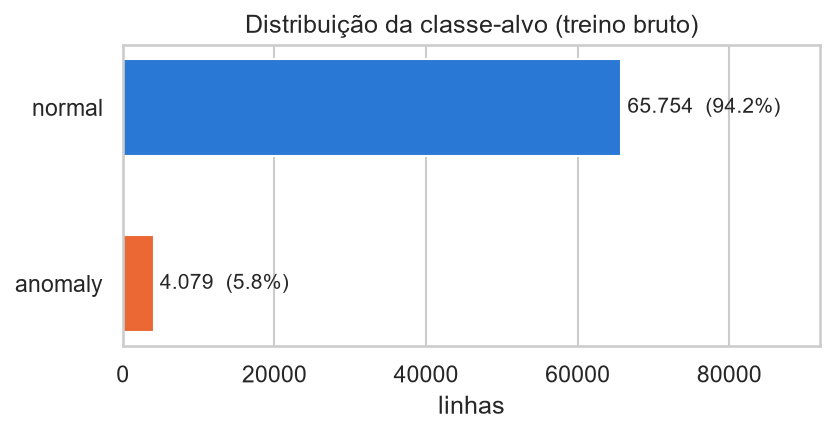
\includegraphics[width=5.57in,height=0.40\textheight,keepaspectratio]{figuras/eda_classes.png}
\caption{Distribuição da classe-alvo no treino bruto.}
\end{figure}

\begin{saida}
razão de desbalanceamento: 16.1:1
'tudo normal': acurácia 0.942, F1-macro 0.485
\end{saida}

Com um desbalanceamento tão forte, a acurácia não diz muito. No F1-macro, a classe \texttt{normal} fica perto de 1 em qualquer modelo razoável, então \textbf{quase toda a diferença entre modelos vem do F1 de \texttt{anomaly}}. Isso torna o \textbf{limiar de decisão} tão importante quanto o balanceamento, e ele será ajustado com previsões \emph{out-of-fold} do treino.

\section{Atributos categóricos}

\begin{figure}[H]
\centering
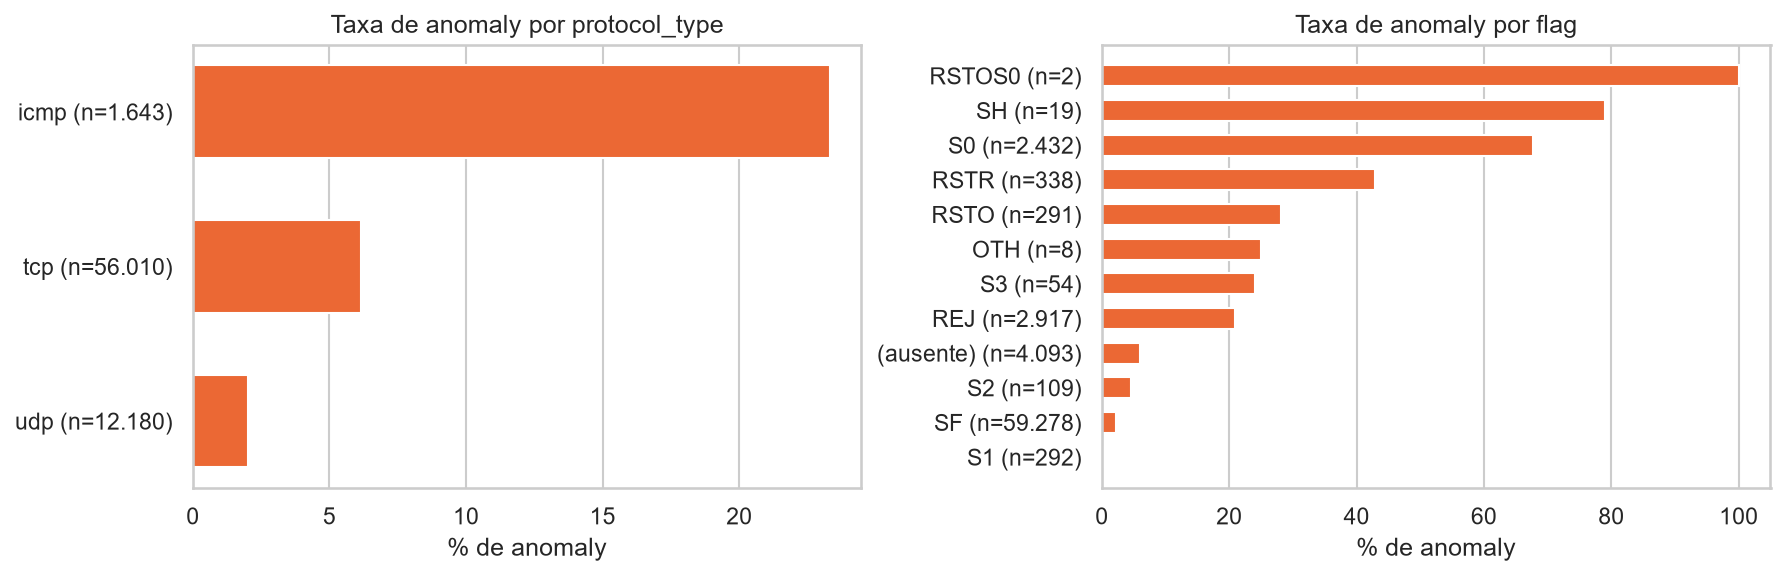
\includegraphics[width=6.50in,height=0.40\textheight,keepaspectratio]{figuras/eda_protocol_flag.png}
\caption{Taxa de anomalia em \texttt{protocol\_type} e \texttt{flag}.}
\end{figure}

O atributo \texttt{flag} separa bem as classes: \texttt{S0} e \texttt{RSTR} concentram anomalias, enquanto \texttt{RSTOS0} e \texttt{SH} têm taxas altas, mas poucas linhas. Quando \texttt{flag} falta, a taxa de anomalia fica próxima da média, então tratamos esse caso como uma categoria própria, chamada \texttt{ausente}.

\begin{saida}
67 serviços; 50 com menos de 0,1% das linhas; os 3 maiores somam 71.5%
\end{saida}

\begin{figure}[H]
\centering
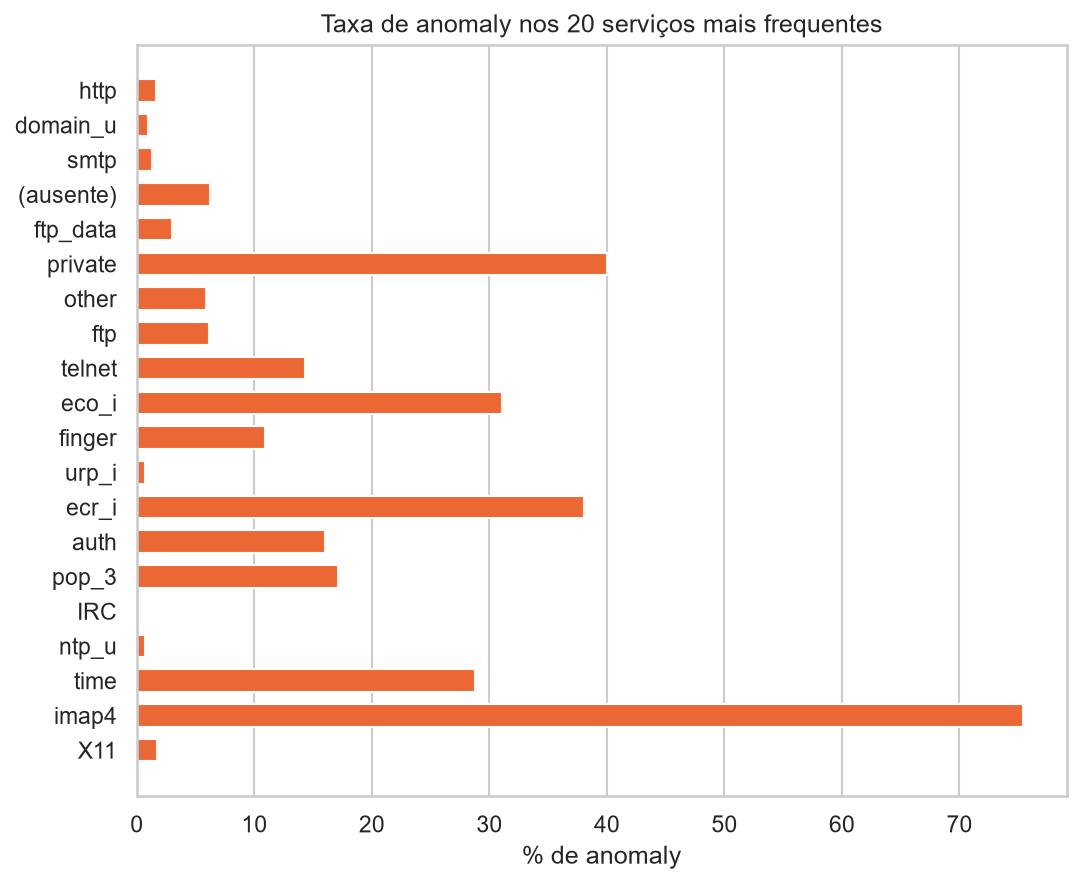
\includegraphics[width=6.50in,height=0.40\textheight,keepaspectratio]{figuras/eda_service_top20.png}
\caption{Taxa de anomalia nos 20 serviços mais frequentes.}
\end{figure}

Já \texttt{service} tem muitos valores raros, e um one-hot criaria quase 70 colunas quase vazias. Por isso, a Etapa 2 compara one-hot, agrupamento dos serviços raros, frequência, \emph{target encoding} com \emph{cross-fitting} e categoria nativa. Como \texttt{protocol\_type} e \texttt{flag} têm poucos valores, ficam em one-hot ou como categoria nativa.

\section{Atributos numéricos e outliers}

\begin{table}[H]
\centering
\caption{Atributos com maior assimetria.}
\begin{adjustbox}{max width=\linewidth}
\begin{tabular}{lrrrr}
\toprule
 & mediana & máximo & skew & \%\_zeros \\
\midrule
dst\_bytes & 365.0 & 209228000.0 & 237.2 & 19.5 \\
num\_root & 0.0 & 7468.0 & 187.5 & 99.2 \\
is\_host\_login & 0.0 & 1.0 & 186.9 & 100.0 \\
urgent & 0.0 & 3.0 & 147.0 & 100.0 \\
src\_bytes & 224.0 & 21945520.0 & 96.7 & 5.6 \\
land & 0.0 & 1.0 & 83.5 & 100.0 \\
num\_file\_creations & 0.0 & 100.0 & 69.2 & 94.4 \\
num\_compromised & 0.0 & 10300.0 & 55.1 & 93.2 \\
\bottomrule
\end{tabular}
\end{adjustbox}
\end{table}

\begin{saida}
constantes: ['num_outbound_cmds']
\end{saida}

\begin{figure}[H]
\centering
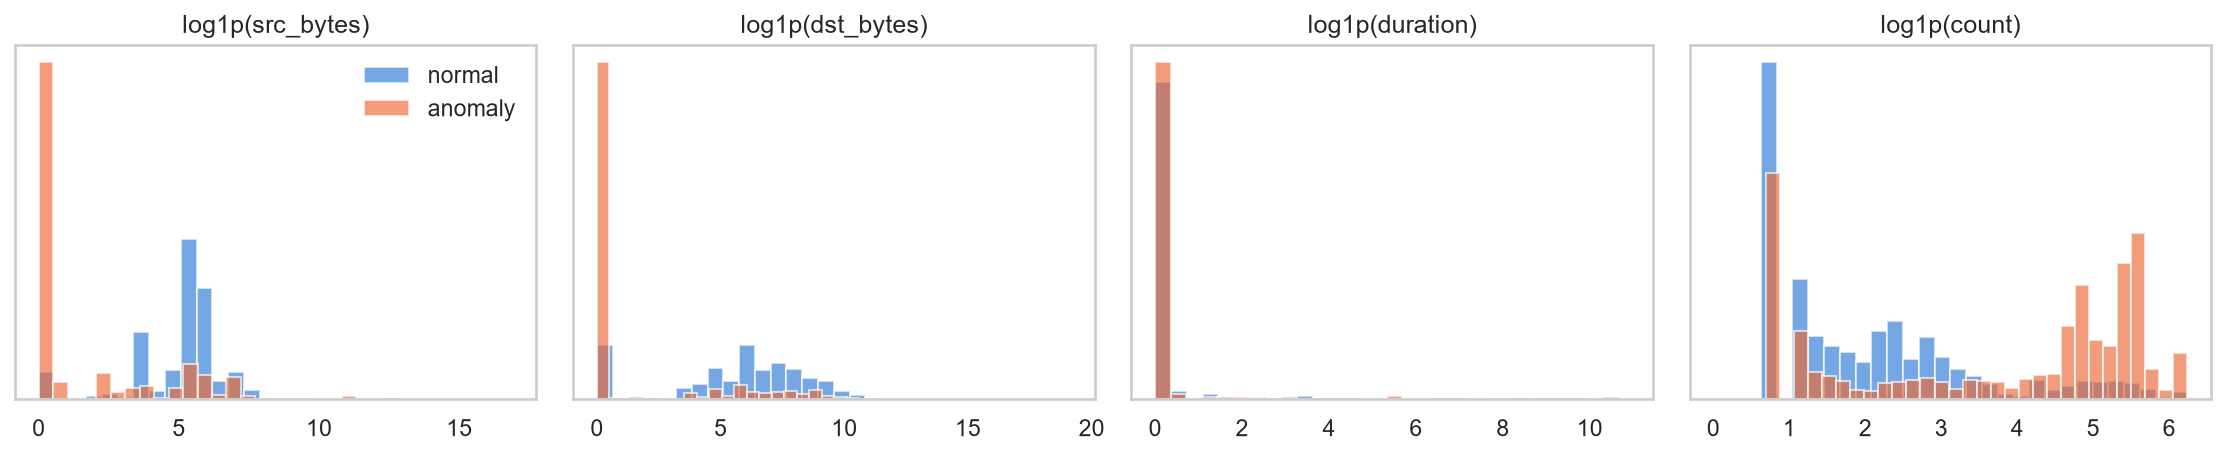
\includegraphics[width=6.50in,height=0.40\textheight,keepaspectratio]{figuras/eda_log_hist.png}
\caption{Histogramas por classe, em escala \texttt{log1p}.}
\end{figure}

Volumes e contagens têm cauda longa: muitos zeros e poucos valores enormes. O \texttt{log1p} comprime essa cauda sem eliminar linhas, o que ajuda MLP, KNN e SMOTE e não muda nada para as árvores. O atributo \texttt{num\_outbound\_cmds} é constante e sai do modelo. Antes de pensar em remover outliers, verificamos o que eles são:

\begin{saida}
linhas com outlier (IQR×3 em log): 14.6%
taxa de anomaly entre outliers: 4.7%; entre os demais: 6.0%
fração das anomalias que uma remoção cega apagaria: 11.8%
\end{saida}

Ao contrário do que se poderia esperar, aqui os outliers \textbf{não} concentram anomalias: são apenas tráfego volumoso legítimo. Removê-los custaria 14,6\% das linhas e 11,8\% das anomalias, sem ganho evidente. Por isso, \textbf{não eliminamos outliers por regra estatística}. Só sai o que é impossível pela definição do atributo.

\section{Redundância de atributos}

\subsection{Colunas novas derivadas}

Cinco colunas novas parecem cálculos feitos sobre atributos existentes. Verificamos se isso é exato e se os ausentes diferem, já que, nesse caso, elas poderiam recuperar valores perdidos:

\begin{table}[H]
\centering
\caption{Igualdade entre as colunas novas e suas fórmulas.}
\begin{adjustbox}{max width=\linewidth}
\begin{tabular}{lrrrr}
\toprule
 & coluna & fórmula & erro\_máx & mesmos\_ausentes \\
\midrule
0 & src\_bytes\_kb & src\_bytes / 1024 & 0.000000e+00 & True \\
1 & dst\_bytes\_kb & dst\_bytes / 1024 & 0.000000e+00 & True \\
2 & total\_bytes & src\_bytes + dst\_bytes & 0.000000e+00 & True \\
3 & same\_srv\_pct & same\_srv\_rate * 100 & 3.552714e-15 & True \\
\bottomrule
\end{tabular}
\end{adjustbox}
\end{table}

\begin{table}[H]
\centering
\caption{\texttt{protocolo\_cod} $\times$ \texttt{protocol\_type}.}
\begin{adjustbox}{max width=\linewidth}
\begin{tabular}{lrrr}
\toprule
protocolo\_cod & 0 & 1 & 2 \\
protocol\_type &  &  &  \\
\midrule
icmp & 0 & 0 & 1643 \\
tcp & 56010 & 0 & 0 \\
udp & 0 & 12180 & 0 \\
\bottomrule
\end{tabular}
\end{adjustbox}
\end{table}

As cinco são \textbf{cópias exatas}, com os mesmos ausentes. Não recuperam nenhum valor e ainda herdam os impossíveis, então \textbf{ficam fora do modelo} (\texttt{config.FEATURES} não as inclui).

\subsection{Correlação entre os 41 atributos}

\begin{saida}
2 pares com |Spearman| > 0,95
\end{saida}

\begin{table}[H]
\centering
\caption{Pares com |Spearman| > 0,95.}
\begin{adjustbox}{max width=\linewidth}
\begin{tabular}{llr}
\toprule
 &  & spearman \\
\midrule
rerror\_rate & srv\_rerror\_rate & 0.951 \\
same\_srv\_rate & diff\_srv\_rate & -0.959 \\
\bottomrule
\end{tabular}
\end{adjustbox}
\end{table}

\begin{figure}[H]
\centering
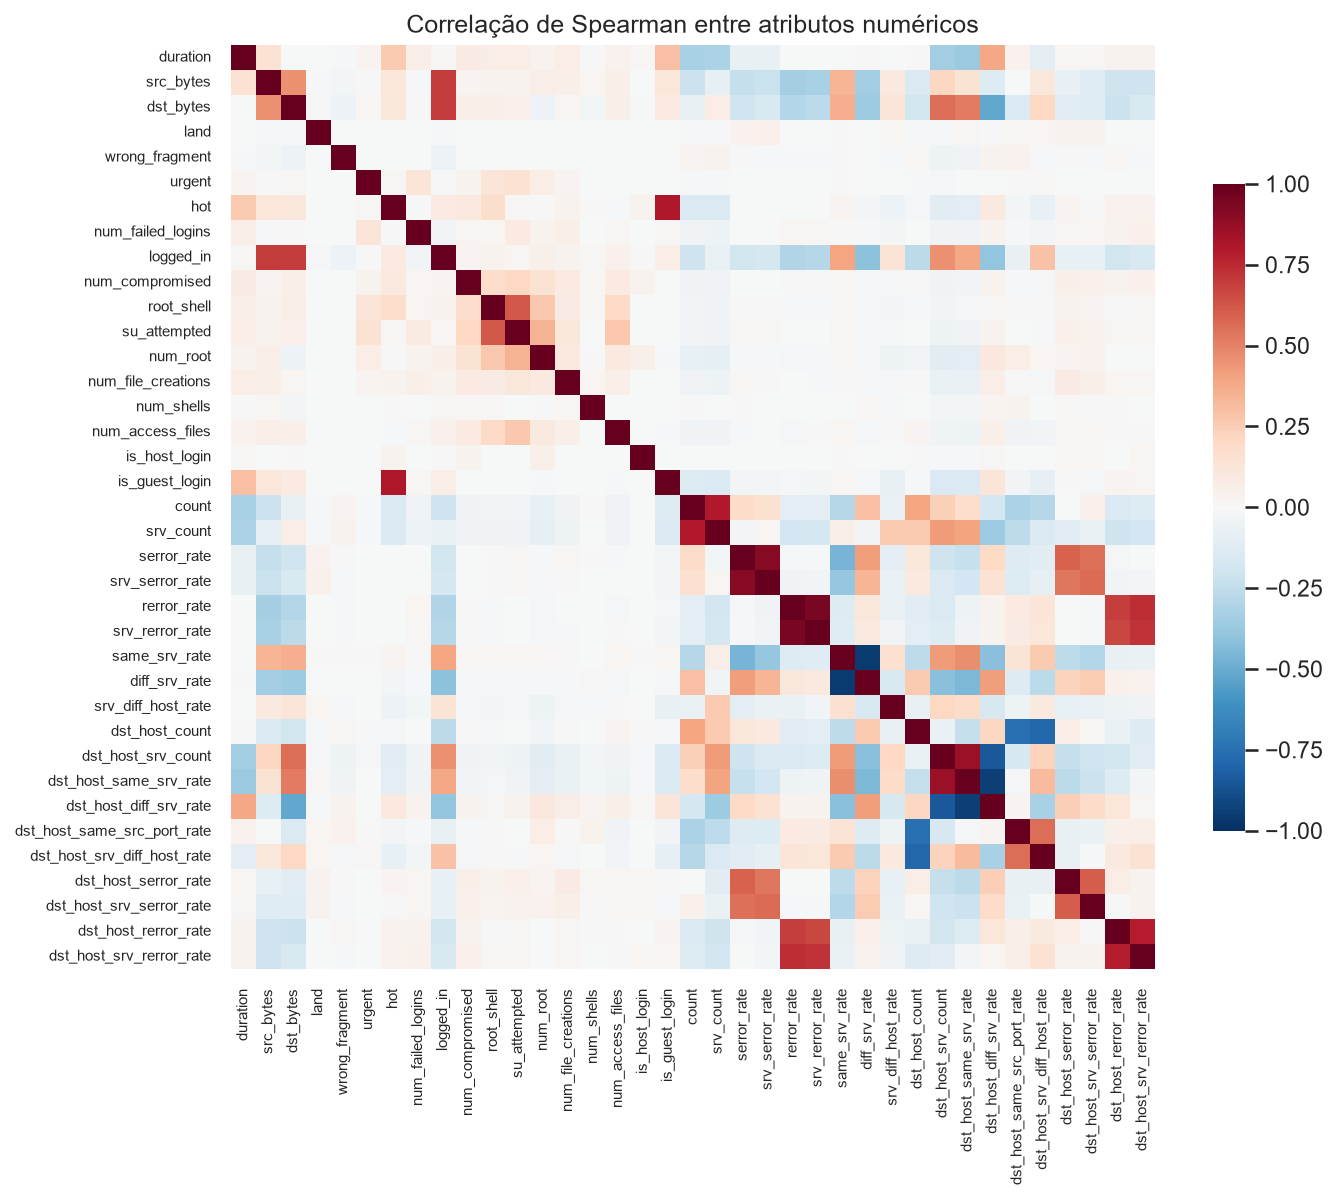
\includegraphics[width=6.50in,height=0.40\textheight,keepaspectratio]{figuras/eda_correlacao.png}
\caption{Correlação de Spearman entre atributos numéricos.}
\end{figure}

\begin{saida}
Pearson serror_rate × srv_serror_rate: 0.973
\end{saida}

Dois pares passam de 0,95. Há um lado bom nisso: como \texttt{srv\_serror\_rate} não tem ausentes, boa parte da informação continua disponível quando \texttt{serror\_rate} falta. A redução de dimensionalidade será comparada na Etapa 2.

\section{Redundância e inconsistência de instâncias}

Aqui olhamos para as linhas, não para as colunas. \textbf{Redundância} é a mesma instância repetida, e \textbf{inconsistência} são instâncias iguais com rótulos diferentes. A comparação usa os 41 atributos, considerando \texttt{NaN} igual a \texttt{NaN}.

\begin{saida}
linhas: 69833  |  linhas distintas: 56766  |  cópias excedentes: 13067
tamanho dos grupos: {1: 44029, 2: 12407, 3: 330}
grupos com rótulos contraditórios: 1702 (3730 linhas)
taxa de anomaly fora dos conflitos: 3.302%; nos conflitos: 50.8%
\end{saida}

Quase 19\% das linhas são cópias, e o fato de os conflitos estarem divididos meio a meio é a marca de rótulos trocados. Isso nos afeta de três formas. Treinar com conflitos ensina o modelo a errar. Na avaliação, nenhuma regra acerta os dois lados de um conflito, já que a mesma linha recebe uma única previsão. Isso cria um teto no F1-macro: mesmo um classificador perfeito fora dos conflitos, que escolhesse o melhor rótulo em cada conflito, ficaria em 0,905. Ainda assim, a métrica oficial é calculada em todas as linhas do teste, e por isso a nossa validação também pontua todas as linhas. E, na validação cruzada comum, as cópias caem em folds diferentes, como discutido na Seção 9.

Para estimar qual seria o rótulo verdadeiro, treinamos um modelo apenas com as linhas sem conflito, sem usar nenhuma coluna suspeita:

\begin{saida}
linhas distintas em conflito: 1702
decididas com confiança (p<0,2 ou p>0,8): 98.5%
estimadas como ataque real: 968 de 1702  |  anomalias sem conflito (linhas distintas): 1817
\end{saida}

O modelo decide com confiança quase todos os casos, e cerca de \textbf{57\% dos conflitos parecem ataques reais}. Descartar todos jogaria fora muitos exemplos positivos, que já são raros. Por isso, a Etapa 2 compara a remoção com a estratégia \texttt{relabel\_model}, que recupera esses casos usando só o fold de treino.

\section{Investigação de vazamento de dados}

\subsection{Associação de cada coluna com a classe}

\begin{table}[H]
\centering
\caption{As 10 colunas mais associadas à classe.}
\begin{adjustbox}{max width=\linewidth}
\begin{tabular}{lrrrrrrr}
\toprule
 & atributo & medida & associacao & info\_mutua & n\_valores & ausentes & alerta \\
\midrule
0 & tipo\_alerta\_soc & cramers\_v & 0.7282 & 0.1215 & 2 & 0.0000 & False \\
1 & score\_ids\_legado & eta & 0.5734 & 0.0994 & 920 & 0.0000 & False \\
2 & flag & cramers\_v & 0.5649 & 0.0690 & 11 & 0.0586 & False \\
3 & service & cramers\_v & 0.5644 & 0.0743 & 67 & 0.0632 & False \\
4 & dst\_host\_srv\_serror\_rate & eta & 0.5363 & 0.0565 & 100 & 0.0399 & False \\
5 & same\_srv\_rate & eta & 0.5225 & 0.0838 & 88 & 0.0511 & False \\
6 & srv\_serror\_rate & eta & 0.5071 & 0.0554 & 56 & 0.0000 & False \\
7 & serror\_rate & eta & 0.4989 & 0.0528 & 51 & 0.0678 & False \\
8 & dst\_host\_serror\_rate & eta & 0.4423 & 0.0246 & 101 & 0.3063 & False \\
9 & tempo\_resposta\_analista\_min & eta & 0.3354 & 0.1112 & 1289 & 0.9137 & False \\
\bottomrule
\end{tabular}
\end{adjustbox}
\end{table}

\begin{figure}[H]
\centering
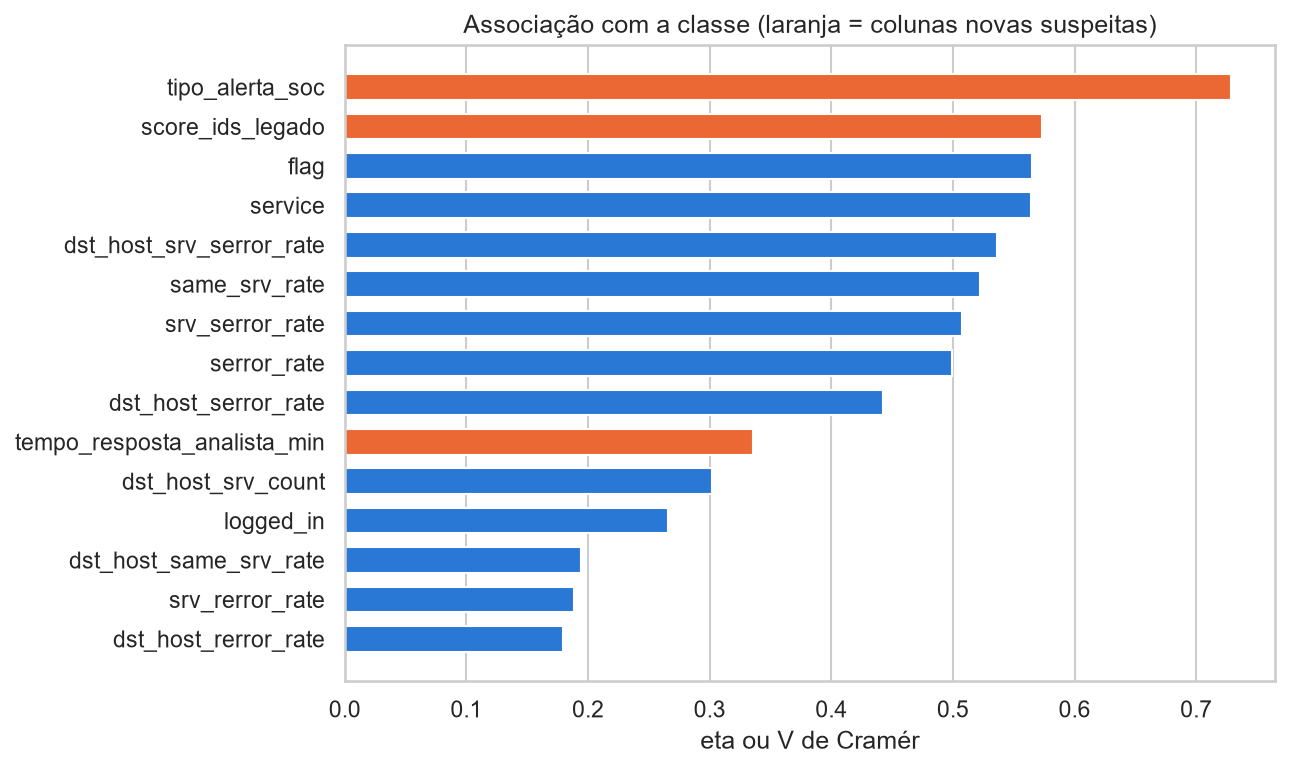
\includegraphics[width=6.50in,height=0.40\textheight,keepaspectratio]{figuras/eda_associacao_classe.png}
\caption{Associação com a classe (laranja: colunas novas suspeitas).}
\end{figure}

As colunas \texttt{score\_ids\_legado} e \texttt{tipo\_alerta\_soc} aparecem acima de todos os atributos de rede. Só isso não prova vazamento, porque atributos legítimos também discriminam. Por isso, investigamos a natureza de cada uma.

\subsection{Elas descrevem o tráfego ou o rótulo?}

\begin{saida}
AUC do score: 0.883
tempo de resposta preenchido: 8.6% das linhas; anomaly quando preenchido: 51.7%; quando vazio: 1.5%
\end{saida}

\begin{table}[H]
\centering
\caption{Classe por score alto e por alerta do SOC.}
\begin{adjustbox}{max width=\linewidth}
\begin{tabular}{llrr}
\toprule
 & classe & anomaly & normal \\
score>0,5 & ALERTA &  &  \\
\midrule
False & False & 0 & 61368 \\
 & True & 83 & 610 \\
True & False & 18 & 1915 \\
 & True & 2082 & 27 \\
\bottomrule
\end{tabular}
\end{adjustbox}
\end{table}

\begin{figure}[H]
\centering
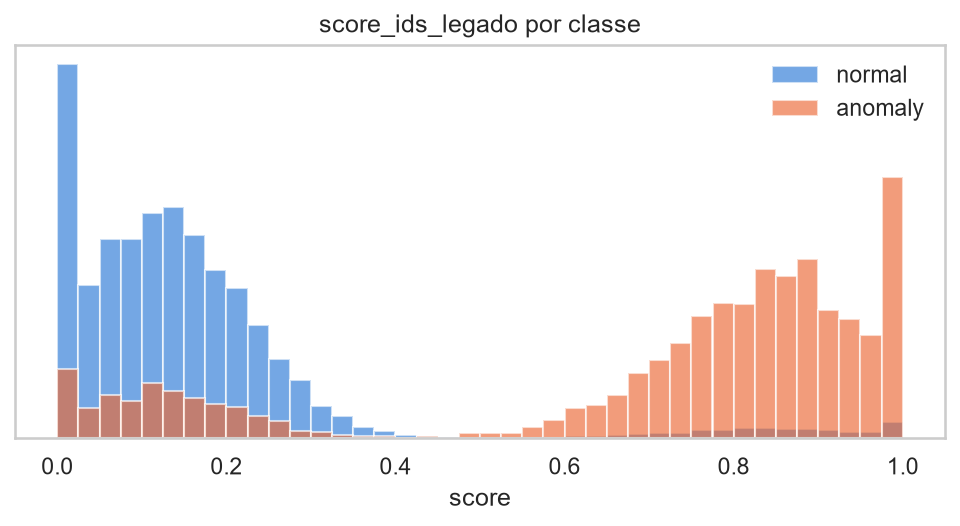
\includegraphics[width=6.40in,height=0.40\textheight,keepaspectratio]{figuras/eda_score_vazamento.png}
\caption{Distribuição de \texttt{score\_ids\_legado} por classe.}
\end{figure}

O caso de \texttt{tempo\_resposta\_analista\_min} é o mais claro: é o tempo que um analista levou para responder depois do evento, algo que não existe no momento de classificar a conexão. Só o fato de estar preenchida muda a taxa de anomalia de 1,5\% para 51,7\%. A coluna \texttt{tipo\_alerta\_soc} também é posterior, pois registra o resultado da triagem do SOC.

Falta decidir sobre \texttt{score\_ids\_legado}, que seria legítimo se fosse a saída de um IDS em operação. Um IDS calcula o score a partir do tráfego, então, entre conexões normais, um score alto deveria corresponder a um tráfego diferente. Testamos isso com um modelo que só vê o tráfego, usando previsões \emph{out-of-fold}:

\begin{table}[H]
\centering
\caption{Probabilidade de ataque vista pelo tráfego, por classe e faixa de score.}
\begin{adjustbox}{max width=\linewidth}
\begin{tabular}{llrrr}
\toprule
 &  & size & mean & median \\
classe & score\_alto &  &  &  \\
\midrule
anomaly & False & 83 & 0.957 & 1.0 \\
 & True & 2100 & 0.935 & 1.0 \\
normal & False & 61978 & 0.001 & 0.0 \\
 & True & 1942 & 0.000 & 0.0 \\
\bottomrule
\end{tabular}
\end{adjustbox}
\end{table}

Entre as conexões \texttt{normal}, ter score alto ou baixo não muda em nada a probabilidade de ataque vista pelo tráfego. Ou seja, o score não está medindo a conexão: ele se comporta como uma \textbf{cópia ruidosa do rótulo}.

\subsection{Quanto cada coluna infla a validação}

\begin{table}[H]
\centering
\caption{F1-macro e AUC por conjunto de colunas, com o mesmo modelo e a mesma validação agrupada, em todas as linhas.}
\begin{adjustbox}{max width=\linewidth}
\begin{tabular}{lrrrr}
\toprule
 & conjunto & n\_colunas & f1\_macro\_cv & auc\_cv \\
\midrule
0 & 41 atributos de rede & 41 & 0.8753 & 0.9033 \\
1 & + score\_ids\_legado & 42 & 0.8842 & 0.9058 \\
2 & + tipo\_alerta\_soc & 42 & 0.8870 & 0.9055 \\
3 & + tempo\_resposta & 42 & 0.8829 & 0.9034 \\
4 & + as três & 44 & 0.8907 & 0.9054 \\
5 & só as três (sem rede) & 3 & 0.8894 & 0.9043 \\
\bottomrule
\end{tabular}
\end{adjustbox}
\end{table}

\textbf{Nossa decisão é manter as três colunas fora do modelo.} Sem nenhum dado de rede, elas alcançam o desempenho do modelo completo (0,889 contra 0,891) e superam os 41 atributos de rede (0,875), o que seria impossível para atributos que realmente descrevem a conexão. Há um sinal ainda mais direto: duas cópias de uma mesma conexão têm o mesmo tráfego, mas as colunas novas variam com o rótulo de cada cópia (nos conflitos, \texttt{tipo\_alerta\_soc} vale ALERTA em 64\% das cópias \texttt{anomaly} e em 56\% das \texttt{normal}). Elas acompanham o rótulo, não a conexão. Em operação, o analista ainda não respondeu e o SOC ainda não fez a triagem, então um detector baseado nelas só detectaria o que já foi detectado.

Como essas colunas também estão no teste, usá-las subiria o ranking, mas o enunciado é claro: vazamento derruba a nota metodológica. A remoção está garantida no código, já que \texttt{config.FEATURES} não as contém e \texttt{tests/test\_leakage.py} verifica isso. Entre os 41 atributos de rede, nenhum passa do alerta de associação de 0,9.

\section{Protocolo de validação}

Antes de comparar técnicas, precisamos de uma régua confiável. Com 19\% de cópias, a validação cruzada comum pode colocar uma linha no treino e sua cópia na validação, testando o modelo em algo que ele já viu. Comparamos as duas abordagens com o mesmo modelo e sem limpeza:

\begin{table}[H]
\centering
\caption{F1-macro por tipo de validação cruzada.}
\begin{adjustbox}{max width=\linewidth}
\begin{tabular}{lrrr}
\toprule
 & CV & f1\_macro (todas as linhas) & sem conflitos (contraste) \\
\midrule
0 & estratificada comum & 0.8698 & 0.9765 \\
1 & agrupada por duplicata & 0.8780 & 0.9756 \\
\bottomrule
\end{tabular}
\end{adjustbox}
\end{table}

As duas réguas discordam, e em direções diferentes conforme as linhas pontuadas. Nas linhas únicas e sem conflito, a validação comum dá um valor um pouco maior (+0,001), porque a cópia da linha validada estava no treino. Em todas as linhas, ela dá um valor \textbf{menor} ($-$0,008): as cópias dos grupos com rótulos contraditórios ficam dos dois lados, e o modelo aprende, para aquela linha exata, o rótulo da cópia que viu no treino, que é o oposto do rótulo de parte das cópias validadas. Nos dois casos, a validação comum mede outra coisa que não a generalização para conexões novas.

O argumento é de correção, não de tamanho: a validação agrupada elimina esse problema por construção e não custa nada. Por isso, o protocolo do trabalho usa \texttt{StratifiedGroupKFold} com o grupo de duplicatas, para que cópias nunca fiquem em lados opostos. A pontuação considera \textbf{todas as linhas} do fold de validação, cópias e conflitos incluídos, porque é assim que a métrica oficial é calculada no teste. O valor nas linhas únicas e sem conflito (\texttt{evaluation\_mask}) é registrado só como contraste: mostra quanto do erro vem do ruído de rótulo, mas não estima a nota. O limiar de decisão é sempre escolhido nos outros folds, nunca naquele que está sendo pontuado.

\section*{Declaração de uso de Inteligência Artificial}
\addcontentsline{toc}{section}{Declaração de uso de Inteligência Artificial}

Declaramos que a ferramenta de Inteligência Artificial Claude
foi utilizada como apoio à revisão crítica das análises e
dos procedimentos desenvolvidos pela equipe, bem como à
formatação e ao aprimoramento da redação deste relatório,
com o objetivo de verificar a consistência do trabalho
realizado e melhorar a clareza, a organização e a
apresentação textual das informações.

\end{document}
